\documentclass[unicode,10pt]{beamer}
\usetheme{ttiposter}

\usepackage{geometry}
\usepackage{luatexja}
\usepackage{graphicx}


\geometry{a4paper,portrait}
\beamertemplatenavigationsymbolsempty

\newcommand{\itemtitle}[1]{\textbf{#1}\\}
\newcommand{\fire}[1]{\textcolor{red}{\textbf{#1}}}
\newcommand{\columnsize}{0.475\textwidth}


\title{文書・文間及びカテゴリ間の関係を考慮したレーティング予測}
\institute{知能数理研究室}
\author{12056 外山 洋太}
\date{\today}



\begin{document}
\begin{frame}
\begin{columns}[onlytextwidth,t]

\begin{column}{\columnsize}
  \begin{block}{背景と目的}
    \begin{itemize}
      \item \itemtitle{商品レビューによる評判分類}
        \begin{itemize}
          \item 対象問題:複数のカテゴリにおける\\レーティング予測
          \item 文字から文書に渡る\fire{様々な言語要素間の関係}、\\
                及び、\fire{カテゴリ間の関係}が重要
          \item 従来手法はそれらを十分に考慮できていない
        \end{itemize}
      \item \itemtitle{目的}
        以下を考慮したレーティング予測の実現
        \begin{itemize}
          \item 文章・文間の関係
          \item カテゴリ間の複雑な関係
        \end{itemize}
    \end{itemize}
    \begin{figure}
      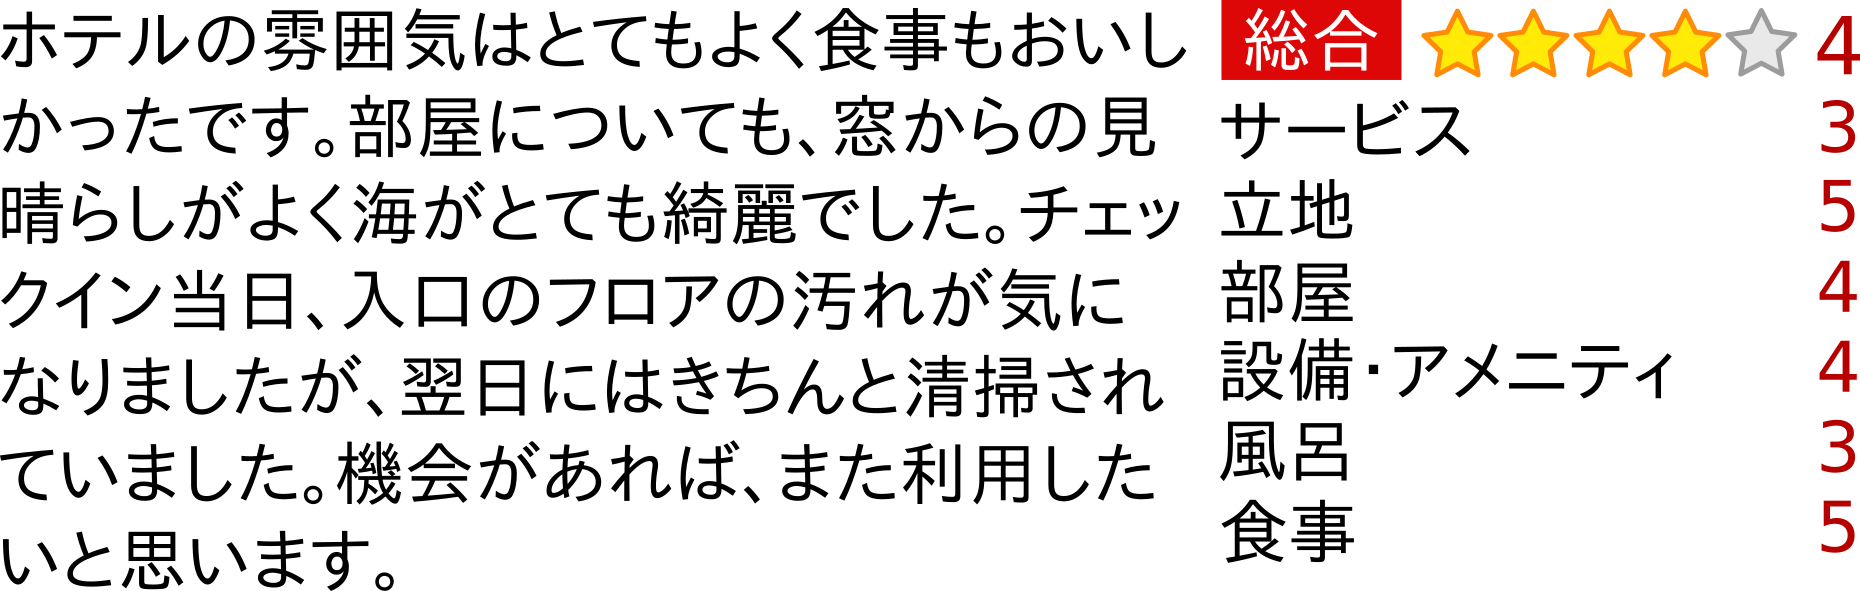
\includegraphics[width=0.9\linewidth]{fig/review.png}
    \end{figure}
  \end{block}

  \begin{block}{関連研究}
    \begin{itemize}
      \item \itemtitle{パラグラフベクトル}
        \begin{itemize}
          \item 文や文書を、その意味を表す実数ベクトルに変換する手法
          \item 評判分類において優れる
        \end{itemize}
      \item \itemtitle{ニューラルネットワーク}
        \begin{itemize}
          \item 神経回路を模した機械学習手法
          \item 分類問題に適用可能
          \item 文書・文間やカテゴリ間の複雑な関係を考慮
        \end{itemize}
    \end{itemize}
  \end{block}

  \begin{block}{提案手法}
    \begin{figure}
      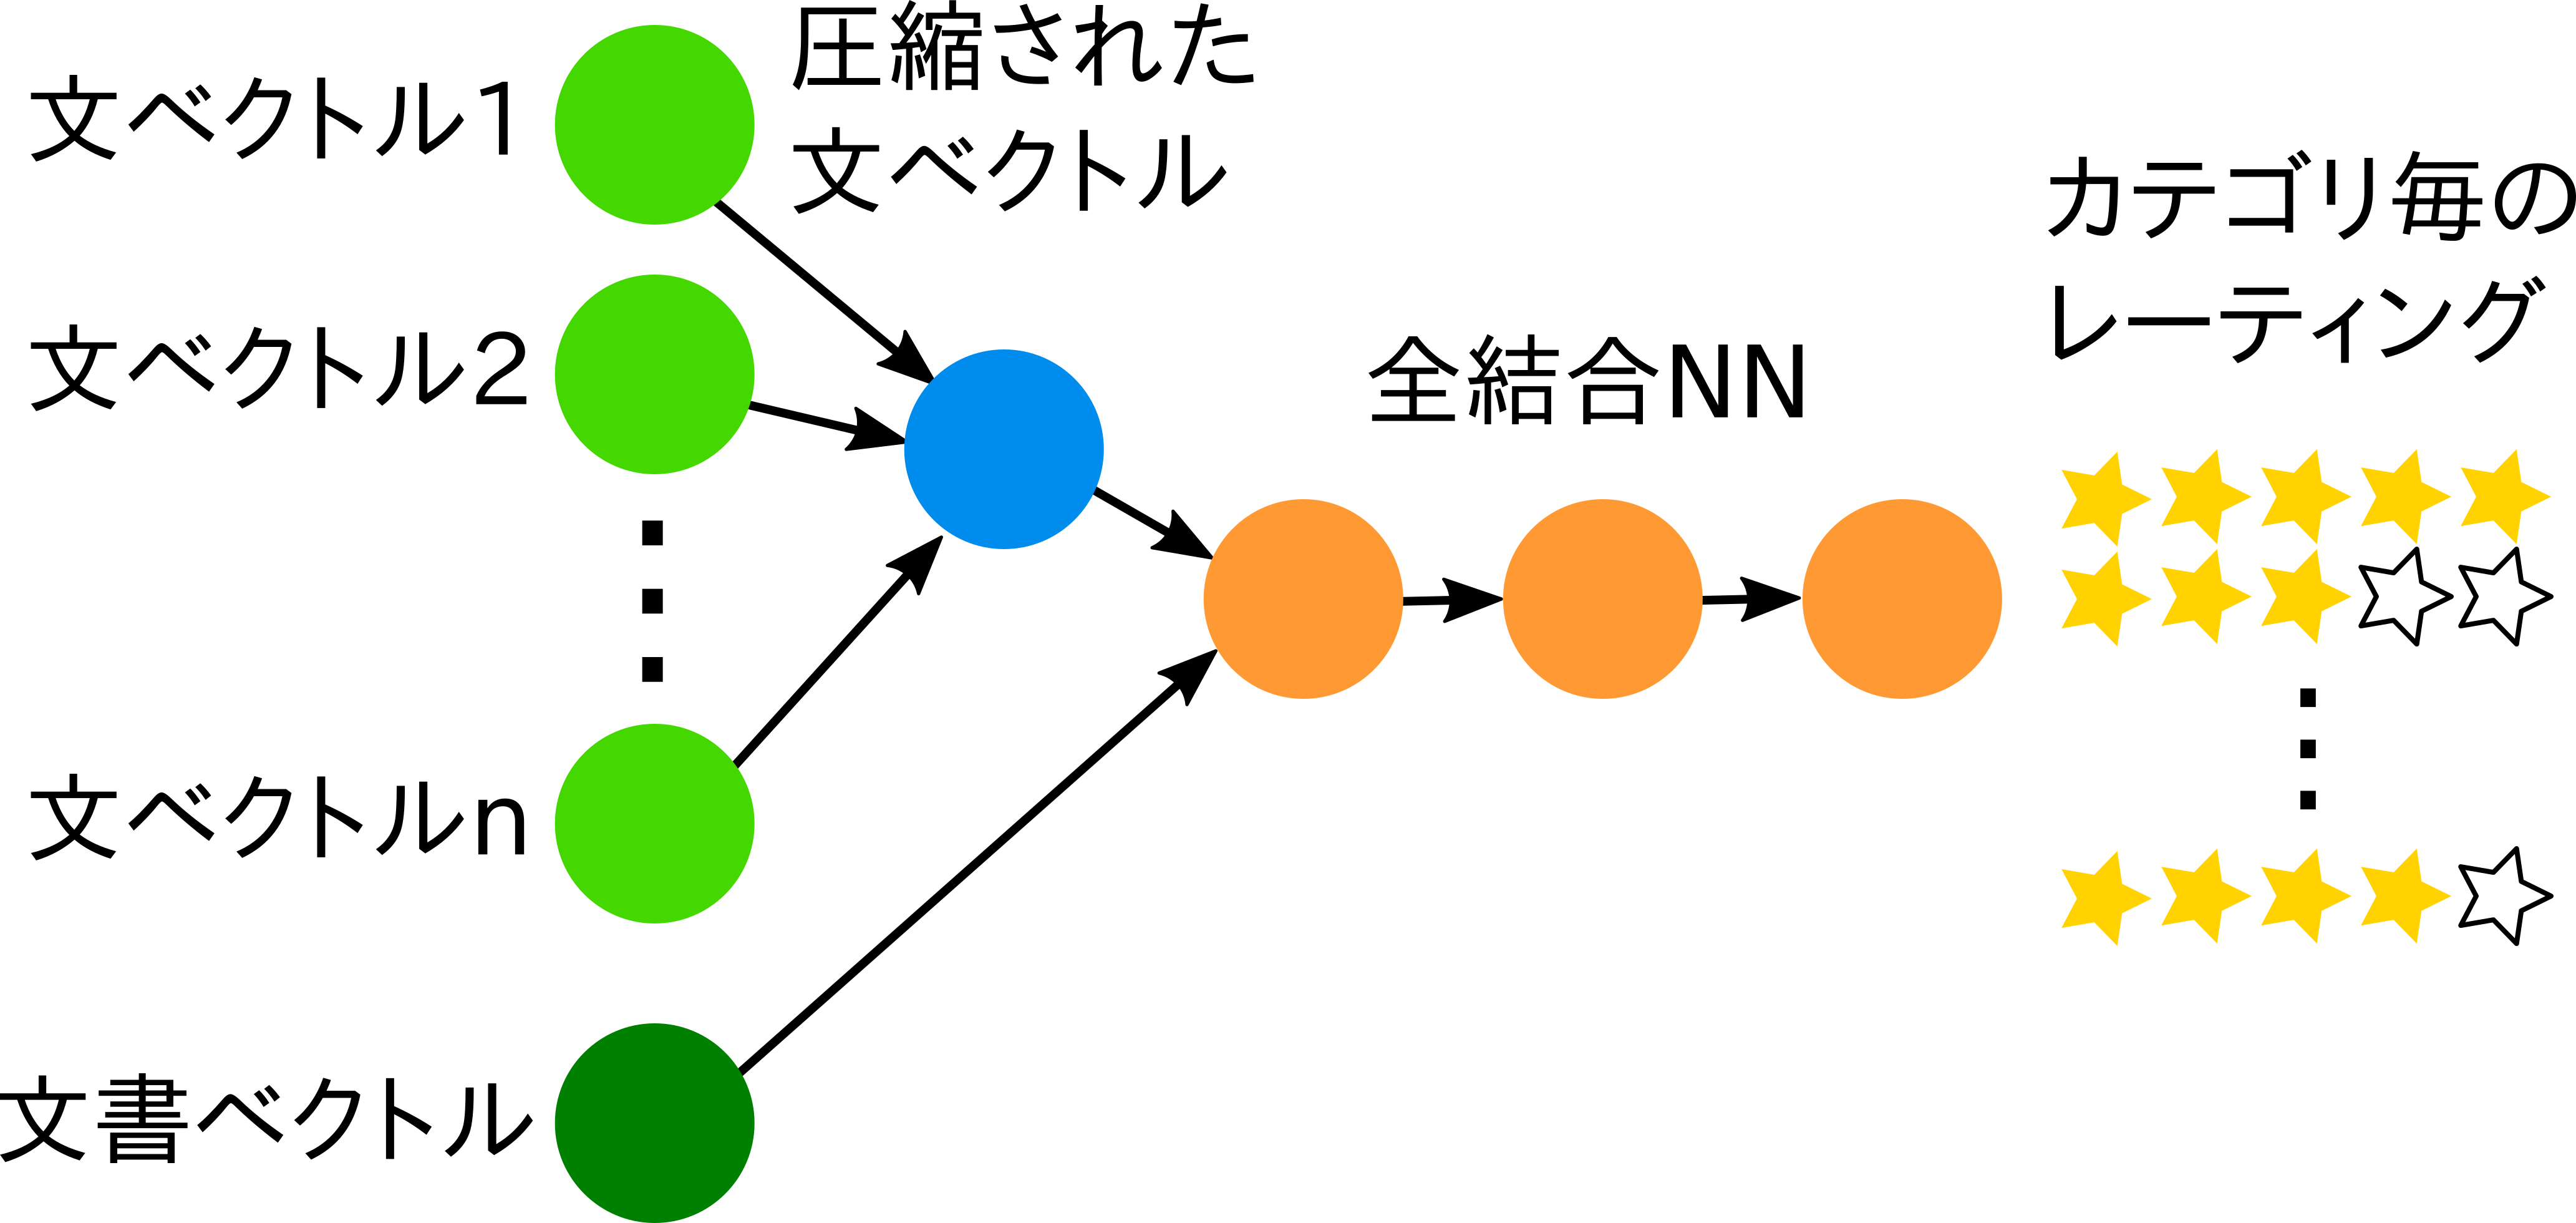
\includegraphics[width=\linewidth]{fig/model.png}
    \end{figure}
  \end{block}
\end{column}

\begin{column}{\columnsize}
  \begin{block}{実験}
    \begin{itemize}
      \item \itemtitle{実験設定}
        \begin{itemize}
          \item 7カテゴリ6クラスのレーティング予測の正答率を測定
          \item データセット:楽天トラベルにおけるレビュー約330,000件
        \end{itemize}
      \item \itemtitle{結果}
        \begin{itemize}
          \item 提案手法が従来手法より\fire{高い正答率}を示す
          \item \fire{文の並び}が予測のために重要
          \item 文書ベクトルと文ベクトルを同時に素性として用いることが有効
        \end{itemize}
    \end{itemize}
    \begin{table}
      \centering
      \begin{tabular}{l | r}
        手法 & 正答率 \\
        \hline
        従来手法 & 0.4832 \\
        提案手法 & \fire{0.5030} \\
      \end{tabular}
    \end{table}
  \end{block}

  \begin{block}{まとめ}
  \end{block}
\end{column}

\end{columns}
\end{frame}
\end{document}
